\chapter{La Magie}
\section{De la Couleur de la Magie}
\label{Couleur}
\subsection{Le cercle des couleurs}
\begin{figure}[h]
    \begin{center}
        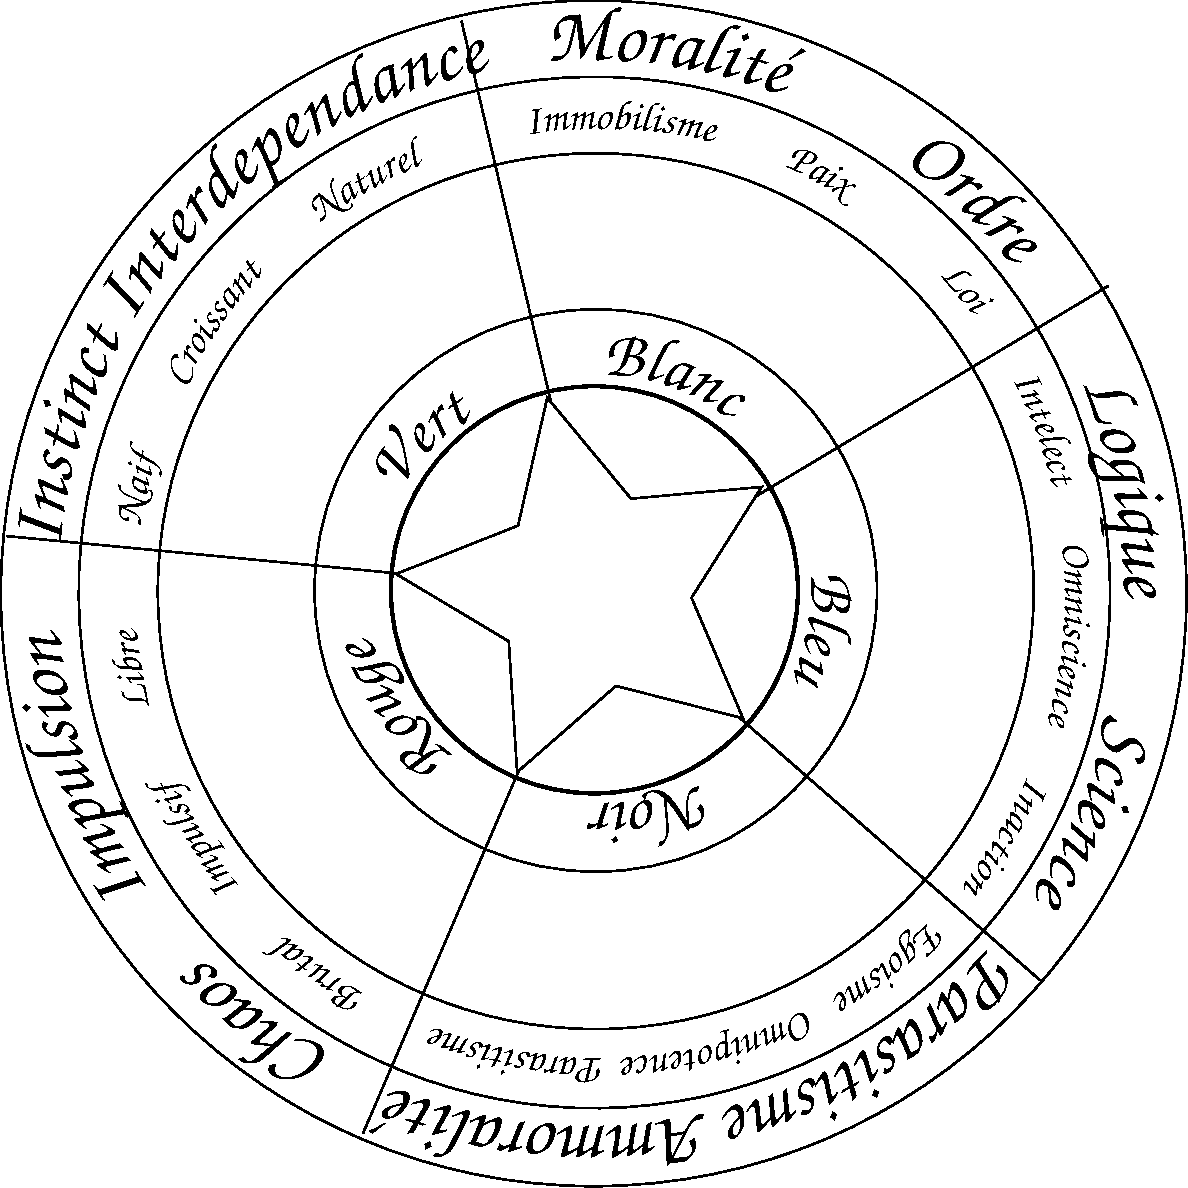
\includegraphics[width=4in,height=4in]{./Images/Circle.pdf}
        \caption{Les cinq couleurs de magie}
    \end{center}
\end{figure}

\subsection{La nature magique des joueur}
Chaque joueur possède lui aussi une nature magique, souvent celle-ci n'as que peu d'importance, 
reflétant seulement une partie de l'état d'esprit du personnage.\\
Cependant elle prendras tout son sens lorsque le personnage sera amené a façonner la réalité de son esprit. 
Dans un souci de cohérence le \Gm pourras conseiller aux joueurs de ce limiter a 2 couleurs.

\section{Les cinq Magies}
\subsection{La {\em Magie innée}}
\subsection{La {\em Haute Magie}}
Un mage est une personne ayant étudié, durant une immense partie de sa vie. 
Sa maîtrise de la magie est telle que chaque sort est d’une réalité très particulière, 
et touche au fondements mêmes de l’univers. Le mage est aux intersections entre réalité et magie, 
il est celui qui déchaîne les forces de l'immatériel au gré de sa volonté.

L’apprentissage de la magie en tant que mage nécessite une compétence représentant la branche de magie étudiée, 
elle représente les connaissances générales dans le domaine le temps passé a étudier, et d'appréhension de cette magie par le mage.

\subsection{La {\em Magie Dragonique}}

\subsection{La {\em Vivemagie}}
\subsection{La {\em Magie Tellurique}}
\section{Les Autres Magies}
\subsection{L'ancienne magie}
\subsection{Les Magies des Plans Extérieurs}
Les magies des plans extérieurs ne peuvent êtres pleinement utilisés sur ce plan.
Cependant la puissance des entités est en telle que celles-ci amènent une partie de leur magie avec elles.
\subsubsection{Invocation}
L'invocation a pour but d'amener totalement ou partiellement une entité des plans extérieurs, vers notre plan d'existence.
Une entité possède plusieurs attributs (\Cf{Les couleurs de Magie}{Couleur}) ainsi qu'un rang divin (\Cf{Classe divine}{Classes}).\\
L'énergie que possédera l'invocation lors de son bref séjour sur ce plan est déterminé comme suit:\\
Le jet lors de l'invocation est ouvert et a la liberté de l'invocateur 
(il choisit lui même a quel tour l'arrêter), le seuil de difficulté est égal au rang de l'entité (il s’agit d’un jet de puissance).
L'entité arrive en jeu avec une énergie égale a l'affinité avec le joueur (a moduler avec les actions de ce dernier) $\times$ Score.
Ce qui représente score/rang minutes de présence, moins les actions effectués, qui coûtent respectivement:
\begin{itemize}
    \item 1 point: Actions banales
    \item 10 point: Actions normales
    \item 20 point: Actions incroyables
    \item 40 point: Actions impossibles
    \item 200 point: Actions demi-divines
\end{itemize}
